\section{System}
\label{sec:sys}

We developed a prototype system \ql which supports \tga operations on
top of Apache Spark/GraphX~\cite{DBLP:conf/osdi/GonzalezXDCFS14}.  The
data is distributed in partitions across the cluster workers, read in
from HDFS, and can be viewed both as a graph and as a pair of RDDs.
All \tg operations are available through the public API of the \ql
library, and may be used in an Apache Spark application.

\subsection{Reducing temporal operators}

Apache Spark is not a temporal DBMS but rather an open-source
in-memory distributed framework that combines graph parallel and data
parallel abstractions.  Following the approach of Dignos et
al.~\cite{Dignos2012} we reduce our temporal operators into a sequence
of nontemporal relational operators or their equivalents for Spark
RDDs, maintaining point semantics.  This allows our algebra to be
implemented in any nontemporal relational database.  In total, we need
the four temporal primitives we introduced in
Section~\ref{sec:algebra:integrity} (coalesce, resolve, constrain, and
split), as well as the primitives described in~\cite{Dignos2012}:
extend and normalize.  Because our model uses point semantics and does
not require change preservation, we do not need the align primitive
of~\cite{Dignos2012} and can use the normalize primitive in its place.

The {\em coalesce} primitive merges adjacent and overlapping time
periods for value-equivalent tuples.  This operation, which is similar
to duplicate elimination in conventional databases, has been
extensively studied in the
literature~\cite{DBLP:conf/vldb/BohlenSS96,DBLP:journals/sigmod/Zimanyi06}.
Several implementations are possible for the coalesce operation over
temporal SQL relations.  Because Spark is an in-memory processing
system, we use the partitioning method, where the relation is grouped
by key, and tuples are sorted and folded within each group to produce
time periods of maximum length.  Eager coalescing, however, is not
desirable since it is expensive and some operations may produce
correct results (up to coalescing) {\em even when computing over
  uncoalesced inputs}.\eat{ We keep track of whether each of the four
  \tve relations is known to be coalesced based on its translation
  into \tra and we include this information in our operator
  definitions in Section~\ref{sec:algebra}.  When an operation
  requires the input to be coalesced, we perform the coalescing on
  each relation as necessary. } Any operation that is time-variant
requires input to be coalesced.\eat{ This includes vertex- and
  edge-subgraph with temporal predicates, node creation with a
  temporal window, aggregation with a temporal predicate, and edge
  creation with a temporal predicate.}  We base the eager coalescing
rules on coalescing rules in \tra~\cite{DBLP:conf/vldb/BohlenSS96}.

\eat{This involves shuffling between partitions, is computationally
  expensive, and motivates lazy coalescing.}

\eat{This was discussed in the context of temporal relational algebra
  in~\cite{DBLP:conf/vldb/BohlenSS96}.}

The {\em resolve} primitive is implemented using a group by key
operation in Spark and convenience methods on the property set class.
The property set class supports adding all properties from another set
such that they are combined by key, and applying aggregation functions
one at a time for each property name.

The {\em constrain} primitive constrains one relation with respect to
another, such as removing edges from the result that do not have
associated nodes, or trimming the edge validity period to be within
the validity periods of associated nodes.  It is introduced here
because Spark does not have a built-in way to express foreign key
constraints.  We do this by executing a join of the two relations ---
either a broadcast join or a hash join --- and then adjusting time
periods as necessary.  This is an expensive operation and is only
performed when necessary as determined by the soundness analysis,
e.g., when vertex-subgraph has a non-trivial predicate over \tve, and
when node creation has a more restrictive vertex quantifier $q_v$ than
edge quantifier $q_e$.

The {\em split} primitive maps each tuple in relation $R$ into one or
more tuples based on a temporal window expression such as
\insql{w=3~months}.  A purely relational implementation of this
primitive is possible with the use of a special Chron relation that
stores all possible time points of the temporal universe and supports
computation without materialization.  Another approach is to introduce
fold and unfold functions that can split each interval into all its
constituent time points.  Both of these approaches have strong
efficiency concerns, see~\cite{DBLP:conf/time/BohlenGJ06} for an
in-depth discussion.  In Spark we are not limited to relational
operators only and can use functional programming constructs.  Split
can be efficiently implemented with a \insql{flatMap}, which emits
multiple tuples as necessary by applying a lambda function and
flattening the result.  We use this method in our implementation.

The {\em extend} primitive extends a relation with an additional
attribute that represents the tuple's timestamp, see~\cite{Dignos2012}
for a definition.  Extend allows explicit references to timestamps in
operations, and is needed for extended snapshot reducibility.  We
implement extend by defining an Interval class and including it as a
field in every RDD.

The {\em normalize} primitive produces a set of tuples for each tuple
in {\bf r} by splitting its timestamp into non-overlapping periods
with respect to another relation {\bf s} and attributes {\bf B}.
See~\cite{Dignos2012} for the formal definition.  Intuitively,
normalize creates tuples in corresponding groups such that their
timestamps are also equivalent.  \eat{For example, for a pair of
  relations $\mathbf{r}$ with single tuple $(v_1, [2016-05-01,
    2016-08-01))$ and $\mathbf{s}$ with single tuple $(v_1,
    [2016-07-01, 2016-09-01))$, it splits the intervals to
      non-overlapping fragments. $\norm{A}{r}{s} = (v_1, [2016-05-01,
        2016-07-01)),(v_1, [2016-07-01, 2016-08-01))$.  }This
        primitive is necessary for node creation, set operators like
        union, and joins.\eat{ Note that Dignos et al. do not use
          $\norm{B}{r}{s}$ for joins, and instead use an align
          operator to support the change preservation property of
          sequenced semantics.}  Normalize primitive relies on an
        efficient implementation of the tuple splitter.  We split each
        tuple based on the change periods over the whole graph,
        avoiding costly joins but potentially splitting some tuples
        unnecessarily.

\subsection{Physical Representations}
\label{sec:sys:datastructs}

\eat{\begin{figure}[t!]
\centering
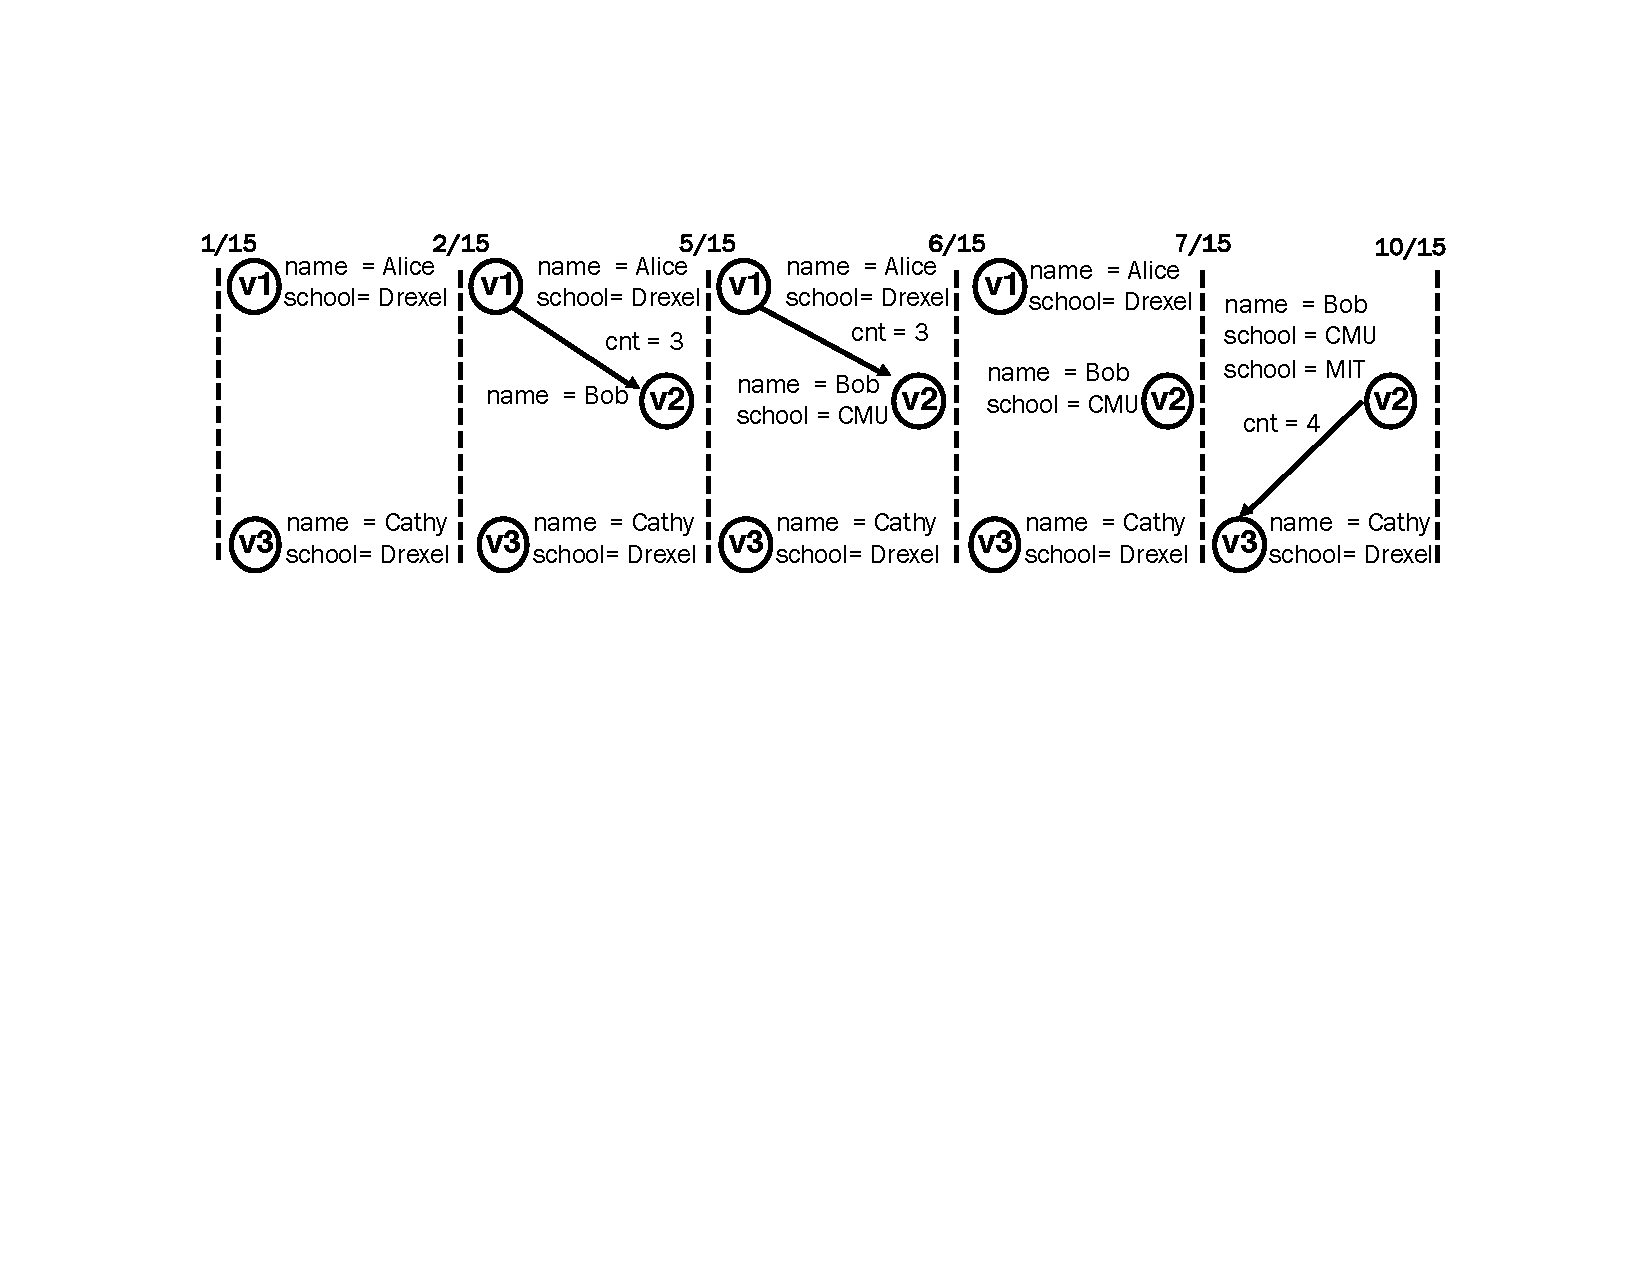
\includegraphics[width=3.4in]{figs/T1_graphs.pdf}
\caption{Representative graphs of \tg \insql{T1}.}
\label{fig:tg_rg}
\end{figure}}

It is convenient to use intervals to compactly represent consecutive
value-equivalent snapshots of \tve --- timeslices in which no change
occurred in graph topology, or in vertex and edge attributes.  We use
the term {\em representative graph} to refer to such snapshots, since
they represent an interval.  \eat{Figure~\ref{fig:tg_rg} shows \insql{T1}
as a sequence of representative graphs.}

We considered four in-memory \tg representations that differ both in
compactness and in the kind of locality they prioritize. With {\em
  structural locality}, neighboring vertices (resp. edges) of the same
representative graph are laid out together, while with {\em temporal
  locality}, consecutive states of the same vertex (resp. edge) are
laid out together~\cite{Miao2015}.  We now
describe each representation.\eat{ VertexEdge (VE) is a direct
  translation of the \ve model of Definition~\ref{def:tg_ve} and the
  most compact representation.  While VE does not necessitate a
  particular order of tuples on disk, we opt for a physical layout in
  which all tuples corresponding to the same vertex (resp. edge) are
  laid out consecutively, and so VE preserves temporal locality.
  RepresentativeGraphs (RG) directly implements the data structure of
  Definition~\ref{def:tg_abstract}, storing each representative graph
  explicitly, and so naturally preserves structural locality, but
  temporal locality is lost.  OneGraph (OG) stores all vertices and
  edges of an evolving graph once, in a single data structure.  This
  representation emphasizes temporal locality, while also preserving
  structural locality.  HybridGraph (HG) trades compactness for better
  structural locality, by aggregating together several consecutive
  RGs, and computing a OneGraph for each RG group.  Details of our
  implementation of the four representations are given below.}

We can convert from one representation to any other at a small cost
(as supported by our experimental results), so it is useful to think
of them as access methods in the context of individual operations.

{\bf VertexEdge (VE)} is a direct implementation of the \tve model,
and is the most compact: one RDD contains all vertices and another all
edges.  Consistently with the GraphX API, all vertex properties are
stored together as a single nested attribute, as are all edge
properties.  We currently do not store the \tv and \te relations
separately but rather together with \tav and \tae, respectively.
While VE does not necessitate a particular order of tuples on disk, we
opt for a physical layout in which all tuples corresponding to the
same vertex (resp. edge) are laid out consecutively, and so VE
preserves temporal locality.

\eat{ The main advantage of this schema-less attribute representation
  is that it can easily deal with schema evolution and leaves the
  details of attribute processing to the user. } 

VE supports all \tga operations except analytics, because an analytic
is defined on a representative graph, which VE does not materialize.
As we will show in Section~\ref{sec:exp}, this physical representation
is the most efficient for many operations.  In the current prototype
we limit the expressiveness of some of the operations, such as only
supporting vertex- and edge-subgraph queries over the \tav and \tae
relations.

{\bf RepresentativeGraphs (RG)} is a collection (parallel sequence) of
GraphX graphs, one for each representative graph of \ttt, where
vertices and edges store the attribute values for the specific time
interval, thus using structural locality.  This representation
supports all operations of \tga which can be expressed over snapshots,
i.e. any operation which does not explicitly refer to time.  GraphX
provides Pregel API which is used to support all the analytics.
%
While the \rg representation is simple, it is not compact, considering
that in many real-world evolving graphs there is a 80\% or larger
similarity between consecutive snapshots~\cite{Miao2015}.  In a
distributed architecture, however, this data structure provides some
benefits as operations on it can be easily parallelized by assigning
different representative graphs to different workers.  We include this
representation mainly as a naive implementation to compare performance
against.

\rg is the most immediate way to implement evolving graphs using
GraphX. Without \ql a user wishing to analyze evolving graphs might
implement and use the \rg approach.  However, as we will show in
Section~\ref{sec:exp}, this would lead to poor performance for most
operations.

\begin{figure}[t!]
\centering
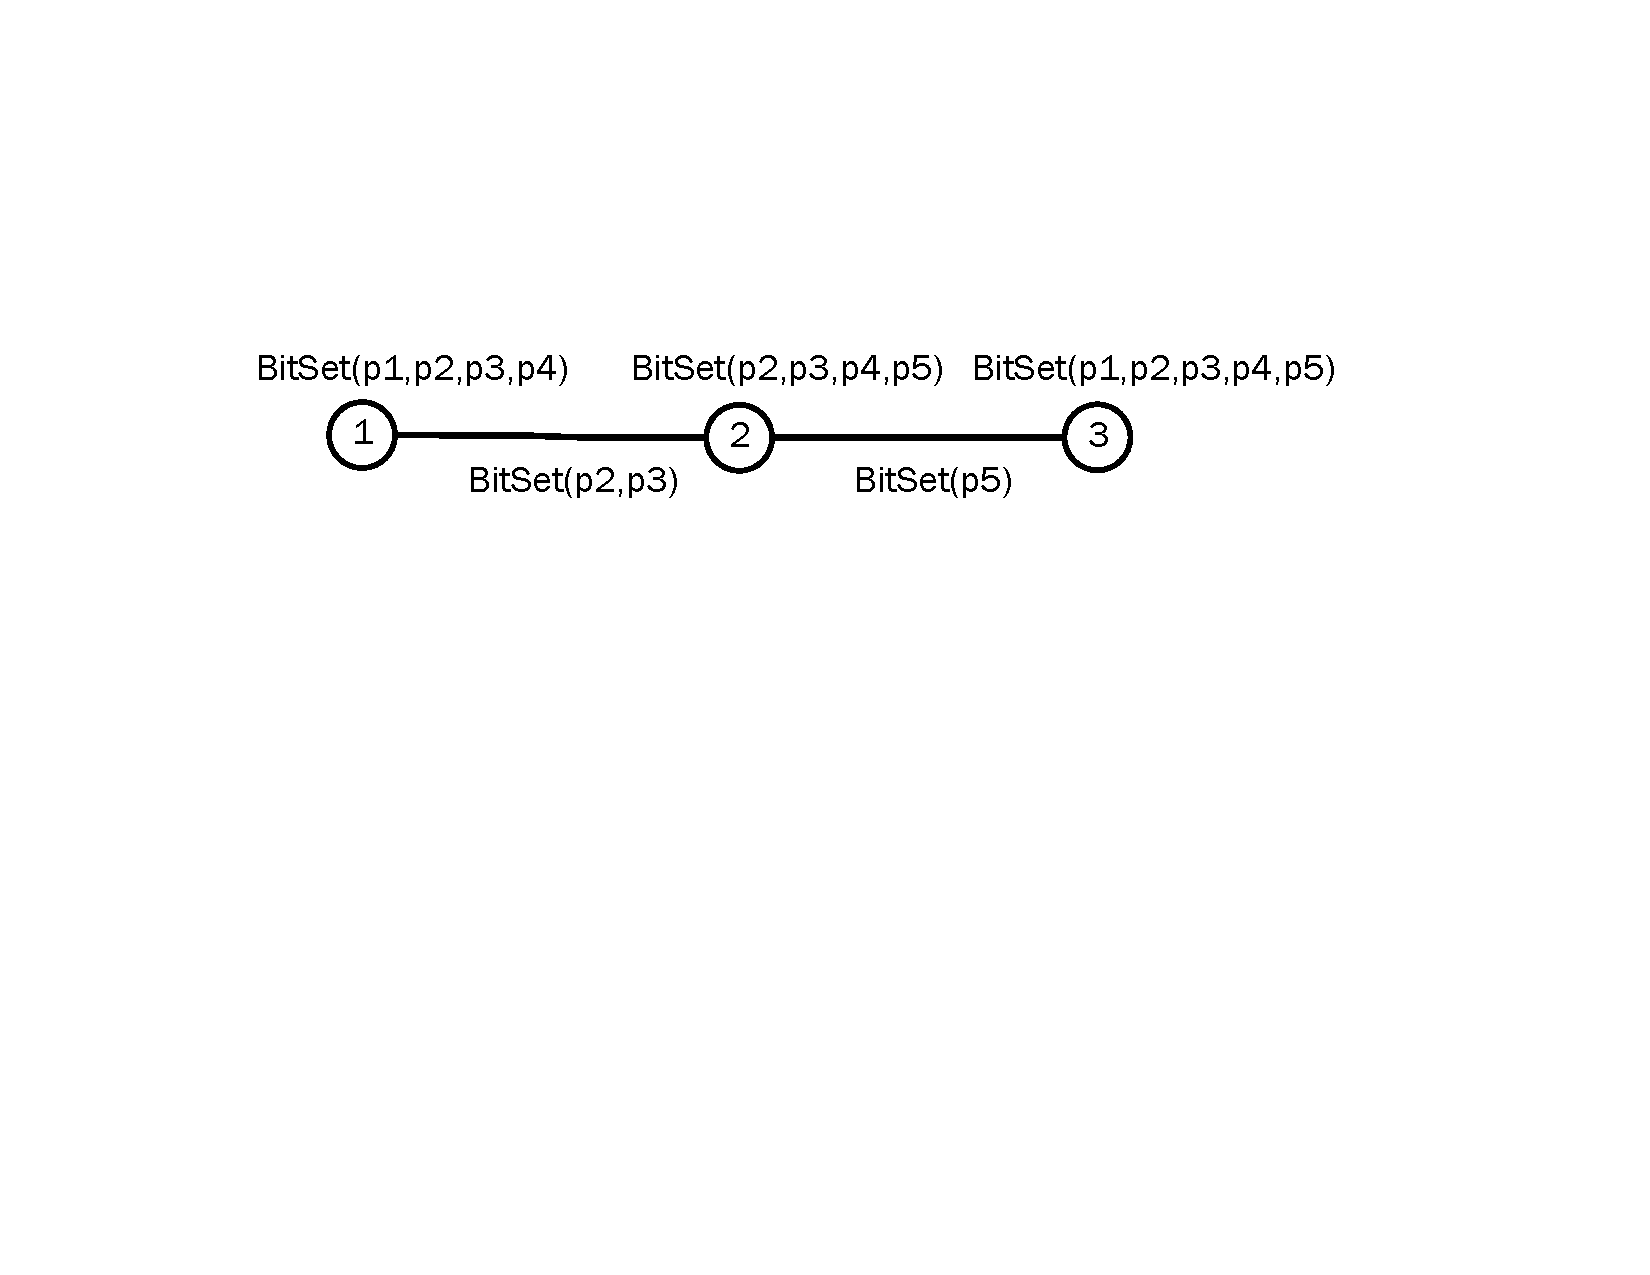
\includegraphics[width=3in]{figs/ogc.pdf}
\vspace{-0.2cm}
\caption{\og representation of \insql{T1}.}
\vspace{-0.1cm}
\label{fig:ogc}
\end{figure}

{\bf OneGraph (OG)} is the most topologically compact representation,
which stores all vertices from \tav {\em and} edges from \tae once, in
a single aggregated data structure.  OG emphasizes temporal locality,
while also preserving structural locality, but leads to a much denser
graph than RG.  This, in turn, makes parallelizing computation
challenging.

An OG is implemented as a single GraphX graph where the vertex and
edge attributes are bitsets that encode the presence of a vertex or
edge in each time period associated with some representative graph of
a \tg.  To construct an \og from \tve, vertices and edges of \tv and
\te relations each are grouped by key and mapped to bits corresponding
to periods of change over the graph.  Because \og stores information
only about graph topology, far fewer periods must be represented and
computed for \og than for \rg.  The actual reduction depends on the
rate and nature of graph evolution.  Information about time validity
is stored together with each vertex and edge.  Figure~\ref{fig:ogc}
shows the OG for \insql{T1} from Figure~\ref{fig:tg_ve}.

Analytics are supported using a batching method over the Pregel API.
Similar to ImmortalGraph~\cite{Miao2015}, the analytics are computed
over all the representative graphs together.  Vertices exchange
messages marked with the applicable intervals and a single message may
contain several interval values as necessary.

As we will see experimentally in Section~\ref{sec:exp}, \og is often
the best-performing data structure for node creation, and also has
competitive performance for analytics.  Because of this focus, \og
supports operations only on topology: analytics, node creation. and
set operators for graphs with no vertex or edge attributes.  All other
operations are supported through inheritance from an abstract parent,
and are carried out on the VE data structure.  Thus \og and \hg,
below, can be thought of as indexes on VE.

In our preliminary experiments we observed that \og exhibited worse
than expected performance, especially for large graphs with long
lifetimes.  The reason this is so is because good graph partitioning
becomes difficult as topology changes over time.  Communication cost
is the main contributor to analytics performance over distributed
graphs, so poor partitioning leads to increased communication costs.
When the whole graph can fit into memory of a single worker,
communication cost goes away and the batching method used by \og
becomes the most efficient, as has been previously shown
in~\cite{Miao2015}.  To provide better performance on analytics, we
introduce {\bf HybridGraph (HG)}.  \hg trades compactness of \og for
better structural locality of \rg, by aggregating together several
consecutive representative graphs, computing a single \og for each
graph group, and storing these as a parallel sequence.  In our current
implementation each \og in the sequence corresponds to the same number
of temporally adjacent graphs.
%
This is the simplest grouping method, and we observed that placing the
same number of graphs into each group often results in unbalanced
group sizes.  This is because evolving graphs commonly exhibit strong
temporal skew, with later graphs being significantly larger than earlier
ones.  We are currently working on more sophisticated grouping
approaches that would lead to better balance, and ultimately to better
performance.  However as we will see experimentally in
Section~\ref{sec:exp}, the current \hg implementation already improves
performance compared to \og, in some cases significantly.

Like \og, \hg focuses on topology-based analysis, and so does not
represent vertex and edge attributes. \hg implements analytics, node
creation, and set operators, and supports all other operations through
inheritance from VE.  Analytics are implemented similar to \og, with
batching within each graph group.

Since RG, OG and HG are implemented over GraphX graphs, the
referential integrity is maintained by the framework and the constrain
primitive is not required.  All primitives are used with the VE
representation.

\subsection{Additional Implementation Details}
\label{sec:sys:maint}

{\bf Partitioning.}  Graph partitioning has a tremendous impact on
performance.  A good partitioning strategy needs to be balanced,
assigning an approximately equal number of units to each partition,
and limit the number of cuts across partitions, reducing
cross-partition communication.  In previous experiments we compared
performance with no repartitioning after load vs.  with
repartitioning, using the GraphX E2D edge partitioning strategy.  In
E2D, a sparse edge adjacency matrix is partitioned in two dimensions,
guaranteeing a $2 \sqrt{n}$ bound on vertex replication, where $n$ is
the number of partitions. E2D has been shown to provide good
performance for Pregel-style
analytics~\cite{DBLP:conf/osdi/GonzalezXDCFS14,MoffittTempWeb16}.  The
user can repartition the representations at will, consistent with the
Spark approach.

{\bf Graph loading.}  We use the Apache Parquet format for on-disk
storage, with one archive for vertices and another for edges,
temporally coalesced.  This format corresponds to the VE physical
representation~\ref{sec:sys:datastructs}.  In cases where there is no
more than 1 attribute per vertex and edge, this representation is also
the most compact.  \eat{If the input data is in uncoalesced snapshots,
  then it occupies space as a function of the graph evolution rate.}

For ease of use, we provide a GraphLoader utility that can initialize
any of the four physical representations from Apache Parquet files on
HDFS or on local disk\eat{, provided that they follow the correct
  schema, using function call
  \insql{GraphLoader.loadDataParquet(\$path)}}.  A \ql user can also
implement custom graph loading methods to load vertices and edges, and
then use the \insql{fromRDDs} to initialize any of the four physical
representations.

{\bf Integration with SQL.}  The \ql API exposes vertex/edge RDDs to
the user and provides convenience methods to convert them to Spark
Datasets.  Arbitrary SparkSQL queries can then be executed over these
relations.

\eat{ We have shown how our logical data model and semantics can be
  implemented in a distributed context. }  

\eat{Next, we show how different physical representations behave on each
operation of \tg algebra.}



